\documentclass[12pt,letterpaper,noanswers]{exam}
\usepackage[usenames,dvipsnames,svgnames,table]{xcolor}
\usepackage[margin=0.9in]{geometry}
\renewcommand{\familydefault}{\sfdefault}
\usepackage{multicol}
\pagestyle{head}
\header{AM 111 Class 04}{}{Linear least squares, p.\thepage}
\runningheadrule
\headrule
\usepackage{siunitx}
\usepackage{enumitem}
\usepackage{graphicx} % more modern
\usepackage{amsmath} 
\usepackage{amssymb} 
\usepackage{hyperref}

\usepackage[most]{tcolorbox}
\usepackage{listings}

\definecolor{white}{rgb}{1,1,1}
\definecolor{mygreen}{rgb}{0,0.4,0}
\definecolor{light_gray}{rgb}{0.97,0.97,0.97}
\definecolor{mykey}{rgb}{0.117,0.403,0.713}

\tcbuselibrary{listings}
\newlength\inwd
\setlength\inwd{1.3cm}
% https://tex.stackexchange.com/questions/340700/ipython-notebook-input-and-output-cells-with-listings
\newcounter{ipythcntr}
\renewcommand{\theipythcntr}{\texttt{[\arabic{ipythcntr}]}}

\newtcblisting{pyin}[1][]{%
  sharp corners,
  enlarge left by=\inwd,
  width=\linewidth-\inwd,
  enhanced,
  boxrule=0pt,
  colback=light_gray,
  listing only,
  top=0pt,
  bottom=0pt,
  overlay={
    \node[
      anchor=north east,
      text width=\inwd,
      font=\footnotesize\ttfamily\color{mykey},
      inner ysep=2mm,
      inner xsep=0pt,
      outer sep=0pt
      ] 
      at (frame.north west)
      {\refstepcounter{ipythcntr}\label{#1}In \theipythcntr:};
  }
  listing engine=listing,
  listing options={
    aboveskip=1pt,
    belowskip=1pt,
    basicstyle=\footnotesize\ttfamily,
    language=Python,
    keywordstyle=\color{mykey},
    showstringspaces=false,
    stringstyle=\color{mygreen}
  },
}
\newtcblisting{pyprint}{
  sharp corners,
  enlarge left by=\inwd,
  width=\linewidth-\inwd,
  enhanced,
  boxrule=0pt,
  colback=white,
  listing only,
  top=0pt,
  bottom=0pt,
  overlay={
    \node[
      anchor=north east,
      text width=\inwd,
      font=\footnotesize\ttfamily\color{mykey},
      inner ysep=2mm,
      inner xsep=0pt,
      outer sep=0pt
      ] 
      at (frame.north west)
      {};
  }
  listing engine=listing,
  listing options={
      aboveskip=1pt,
      belowskip=1pt,
      basicstyle=\footnotesize\ttfamily,
      language=Python,
      keywordstyle=\color{mykey},
      showstringspaces=false,
      stringstyle=\color{mygreen}
    },
}
\newtcblisting{pyout}[1][\theipythcntr]{
  sharp corners,
  enlarge left by=\inwd,
  width=\linewidth-\inwd,
  enhanced,
  boxrule=0pt,
  colback=white,
  listing only,
  top=0pt,
  bottom=0pt,
  overlay={
    \node[
      anchor=north east,
      text width=\inwd,
      font=\footnotesize\ttfamily\color{mykey},
      inner ysep=2mm,
      inner xsep=0pt,
      outer sep=0pt
      ] 
      at (frame.north west)
      {\setcounter{ipythcntr}{\value{ipythcntr}}Out#1:};
  }
  listing engine=listing,
  listing options={
      aboveskip=1pt,
      belowskip=1pt,
      basicstyle=\footnotesize\ttfamily,
      language=Python,
      keywordstyle=\color{mykey},
      showstringspaces=false,
      stringstyle=\color{mygreen}
    },
}





\newcommand{\note}[1]{\textcolor{red}{#1}} % show notes in red
\renewcommand{\note}[1]{} % don't display notes

\begin{document}
 \pdfpageheight 11in 
  \pdfpagewidth 8.5in

\noindent 

\note{calendar:
\begin{enumerate}
    \item Tu binary subtraction, least sq intro PS01/2
    \item Th least sq PS02
    \item Tu lin alg PS02/3
    \item Th lin alg PS03
    \item Tu least sq PS03/4
    \item Th ?? PS04
    \item Tu root finding PS04/5
    \item Th root finding PS05 (early)
    \item Tu integration PS06
    \item Th quiz
    \item Tu interpolation PS06
    \item Th interpolation PS06
    \item Tu integration PS07
    \item Th Monte Carlo PS07
    \item Tu differentiation PS08
    \item Th differentiation PS08
    \item Tu diff eq
    \item Th application of diff eq
    \item Tu ODEs
    \item Th ODEs
    \item Tu neural nets
    \item Tu neural nets
    \item Th quiz
    \item Tu presentations
\end{enumerate}}

\note{
\begin{itemize}
    \item what is a floating point system
    \item example
    \item IDing info about a floating point system
    \item 
\end{itemize}
}
\setcounter{section}{-1}
\section{Preliminaries}
\begin{itemize}
\itemsep0pt
\item There will be a skill check in class during the next class.  The problem info is below.
\item Problem set 01 is due on Friday.
\item There is a reading assignment for Tuesday.
\end{itemize}

\hrule
\vspace{0.2cm}


\noindent\textbf{Big picture}
\begin{itemize}
    \itemsep0pt
\item How do we solve a linear least squares problem?
\item How do we measure the sensitivity of a problem to small errors?
\end{itemize}

\vspace{0.2cm}
\hrule
\vspace{0.2cm}

\noindent \textbf{Skill check practice}

Set up a model, written in matrix form, for finding a parabola, $y = c_1 + c_2 t + c_2 t^2$, through the data points $(-1,1), (0,0)$, $(1,0), (2,-2)$.

\emph{Do not create the normal equations.}



\vspace{0.2cm}
\hrule
\vspace{0.2cm}

\noindent \textbf{Skill check solution}

The $y$ values go on the right hand side.  On the left hand side, the $A$ matrix has columns $1$, $t$, $t^2$.  The unknown coefficients are $c_1, c_2, c_3$.

$\left[\begin{array}{c c c}1 & -1 & 1 \\
1 & 0 & 0 \\
1 & 1 & 1 \\
1 & 2 & 4\end{array}\right]\left[\begin{array}{c}c_1\\c_2\\c_3\end{array} \right]= \left[\begin{array}{c}1 \\ 0 \\ 0 \\ -2\end{array}\right]$


\vspace{0.2cm}
\hrule
\vspace{0.2cm}

\section{Lower dimensional representations}
\subsection{Cost functions}

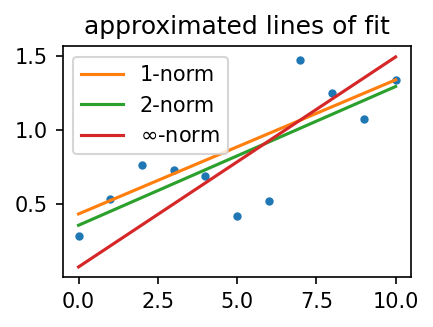
\includegraphics{AM111-F23-CourseNotes/img/c04-line.png}

\begin{enumerate}
\itemsep50pt
\item Based on the Python code that was used to generate this figure (shared via projector), what was the method for finding the coefficients of each best fit line?
\item Will that method yield the linear least squares solution when the $2$-norm is used?  Why or why not?
\end{enumerate}
\vspace{1in}


\begin{enumerate}[resume]
\itemsep80pt
\item In the $x_1x_2$-plane, let  $\mathbf{v}=(x_1,x_2)$.  
\begin{parts}
\itemsep80pt
\item Set up an equation describing the set of points in the plane so that $\Vert\mathbf{v}\Vert_2 = 1$ (and sketch the set of points).
\item Set up one or more equations describing the set of points in the plane so that $\Vert\mathbf{v}\Vert_1 = 1$  (and sketch the set of points).
\item Set up one or more equations describing the set of points in the plane so that $\Vert\mathbf{v}\Vert_{\infty} = 1$  (and sketch the set of points).
\end{parts}
\vspace{1.5in}
\end{enumerate}



\section{Linear least squares}


\begin{enumerate}[resume]
\itemsep50pt
\item Consider the data $\{(0,3),(1,2),(2,4)\}$.  We wish to fit a line, $c_1 + c_2 t = y$.
\begin{parts}
\itemsep50pt
\item Write the problem in matrix form.

\emph{Write out all known values in the matrix equations}
\item There are $N=3$ data points and $M=2$ basis functions.  What are the dimensions of $A$, $\textbf{c}$, and $\textbf{y}$ in terms of $M$, $N$, and $1$?
\item Why isn't there a solution to the system $A\mathbf{c} = \mathbf{y}$?
\end{parts}
%\eject

\item Find the associated normal equations, $A^TA\overline{\mathbf{c}} = A^T\mathbf{y}$.  \emph{Do any matrix multiplication to simplify.}
\end{enumerate}

\vspace{1in}

\begin{enumerate}[resume]
\itemsep50pt
    \item The Python code below was used to add a linear least squares curve fit to the temperature data on the first page.  The following questions are about the code.
    \begin{parts}
    \itemsep50pt
    \item What are the columns of the regression matrix?  What are the steps used to construct the regression matrix in this code?
    \item What is the role of $\omega$ (\texttt{omega})?  Why is it $2\pi/365$?
    \item What do you learn about the temperature data from these curves of fit?  What would you need to do to find the amplitude and phase of the sinusoidal fit?
    \end{parts}

    \vspace{1in}
\end{enumerate}
\begin{verbatim}
import numpy as np
# data is in xv and yv.

# least squares fit
omega = 2*np.pi/365
A = np.vstack([np.ones(len(xv)), np.cos(omega*xv), np.sin(omega*xv)]).T
alpha = np.linalg.lstsq(A, yv, rcond=None)[0]
\end{verbatim}

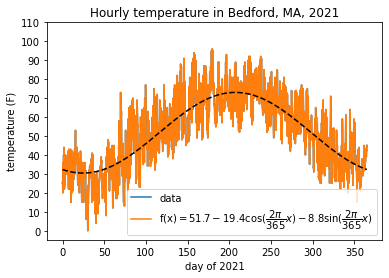
\includegraphics[width=0.45\linewidth]{img/C03weatherBedfordfit.png}
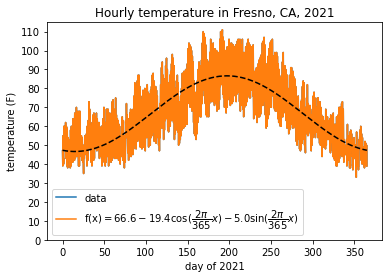
\includegraphics[width=0.45\linewidth]{img/C03weatherFresnofit.png}

\subsection{Normal equations}
\begin{enumerate}[resume]
    \item Given a dataset with $m$ pairs, and a model with $n$ parameters, identify the dimensions of $A^TA$, $\mathbf{c}$, and $A^T\mathbf{y}$.    
\end{enumerate}
\vspace{1in}
\section{Error due to approximations}

\begin{enumerate}[resume]
\itemsep50pt
\item
Consider $y = f(x)$ for some function $f$.  If the condition number is $\approx 1$, and you change your input value by $1\%$, how do you expect the output value to change?

\vspace{0.5in}

\item
What if the condition number is $100$?  In this case, if you change your input value by $1\%$, how do you expect the output value to change?

\vspace{0.5in}
\end{enumerate}

\end{document}